\documentclass[aspectratio=169,10pt]{beamer}

\usepackage[T1]{fontenc}
\usepackage[utf8]{inputenc}
\usepackage[brazilian]{babel}
\usepackage{lmodern}
\usepackage{booktabs}
\usepackage{tabularx}
\usepackage{array}
\usepackage{amsmath}
\usepackage{csquotes}
\usepackage{tikz}
\usetikzlibrary{arrows.meta,positioning}

\usetheme[progressbar=frametitle,numbering=fraction]{metropolis}
\definecolor{verde}{HTML}{1F9D55}
\definecolor{escuro}{HTML}{1B2430}
\definecolor{vermelho}{HTML}{C0392B}
\setbeamercolor{frametitle}{bg=escuro,fg=white}
\setbeamercolor{progress bar}{fg=verde,bg=escuro!30}
\setbeamercolor{title separator}{fg=verde}
\setbeamercolor{alerted text}{fg=vermelho}
\setbeamercolor{block title}{bg=verde!15,fg=escuro}
\setbeamercolor{block body}{bg=verde!5}

\newcolumntype{L}{>{\raggedright\arraybackslash}X}
\newcommand{\credito}[1]{{\tiny\color{gray}#1}}
\newcommand{\ideia}[1]{\par\vfill\noindent\colorbox{verde!12}{\parbox{\dimexpr\linewidth-2\fboxsep\relax}{\small\strut #1\strut}}}

\tikzset{
  caixa/.style={draw=escuro, rounded corners, align=center, minimum height=0.9cm, inner sep=3pt, fill=white, font=\small},
  seta/.style={-{Stealth}, thick, color=escuro}
}

\title{HIJACK: carrinho hackeável para o ensino de cibersegurança}
\subtitle{Fundamentos de Circuitos e Sistemas Controlados}
\author{\scriptsize
\begin{tabular}{@{}ll@{}}
Pedro Nascimento de Paiva Fernandes Neto & Marcelo Jorge Oliveira de Albuquerque Melo \\
Carlos Roberto de Miranda Gomes Neto & Matheus Felipe Duarte Dionísio \\
Élisson Rian Félix Simas & João Gonçalves de Souza Neto \\
Gustavo Henrique Assunção Paiva & \\
\end{tabular}}
\institute{\small Universidade Federal do Rio Grande do Norte (UFRN)\\Professor: Alexandre Magnus Fernandes Guimarães}
\date{\small Natal, novembro de 2026}

\begin{document}

\begin{frame}[plain]
\begin{columns}[c]
\column{0.58\textwidth}
{\LARGE\bfseries\color{escuro} HIJACK}\\[2pt]
{\large Carrinho hackeável para o ensino de cibersegurança}\\[-2pt]
{\color{verde}\rule{\linewidth}{1.2pt}}\\[4pt]
\scriptsize
Pedro Nascimento de Paiva Fernandes Neto\\
Carlos Roberto de Miranda Gomes Neto\\
Élisson Rian Félix Simas\\
Gustavo Henrique Assunção Paiva\\
Marcelo Jorge Oliveira de Albuquerque Melo\\
Matheus Felipe Duarte Dionísio\\
João Gonçalves de Souza Neto\\[8pt]
\footnotesize
\textbf{Fundamentos de Circuitos e Sistemas Controlados}\\
Professor: Alexandre Magnus Fernandes Guimarães\\
Universidade Federal do Rio Grande do Norte (UFRN)\\
Natal, novembro de 2026
\column{0.4\textwidth}
\centering
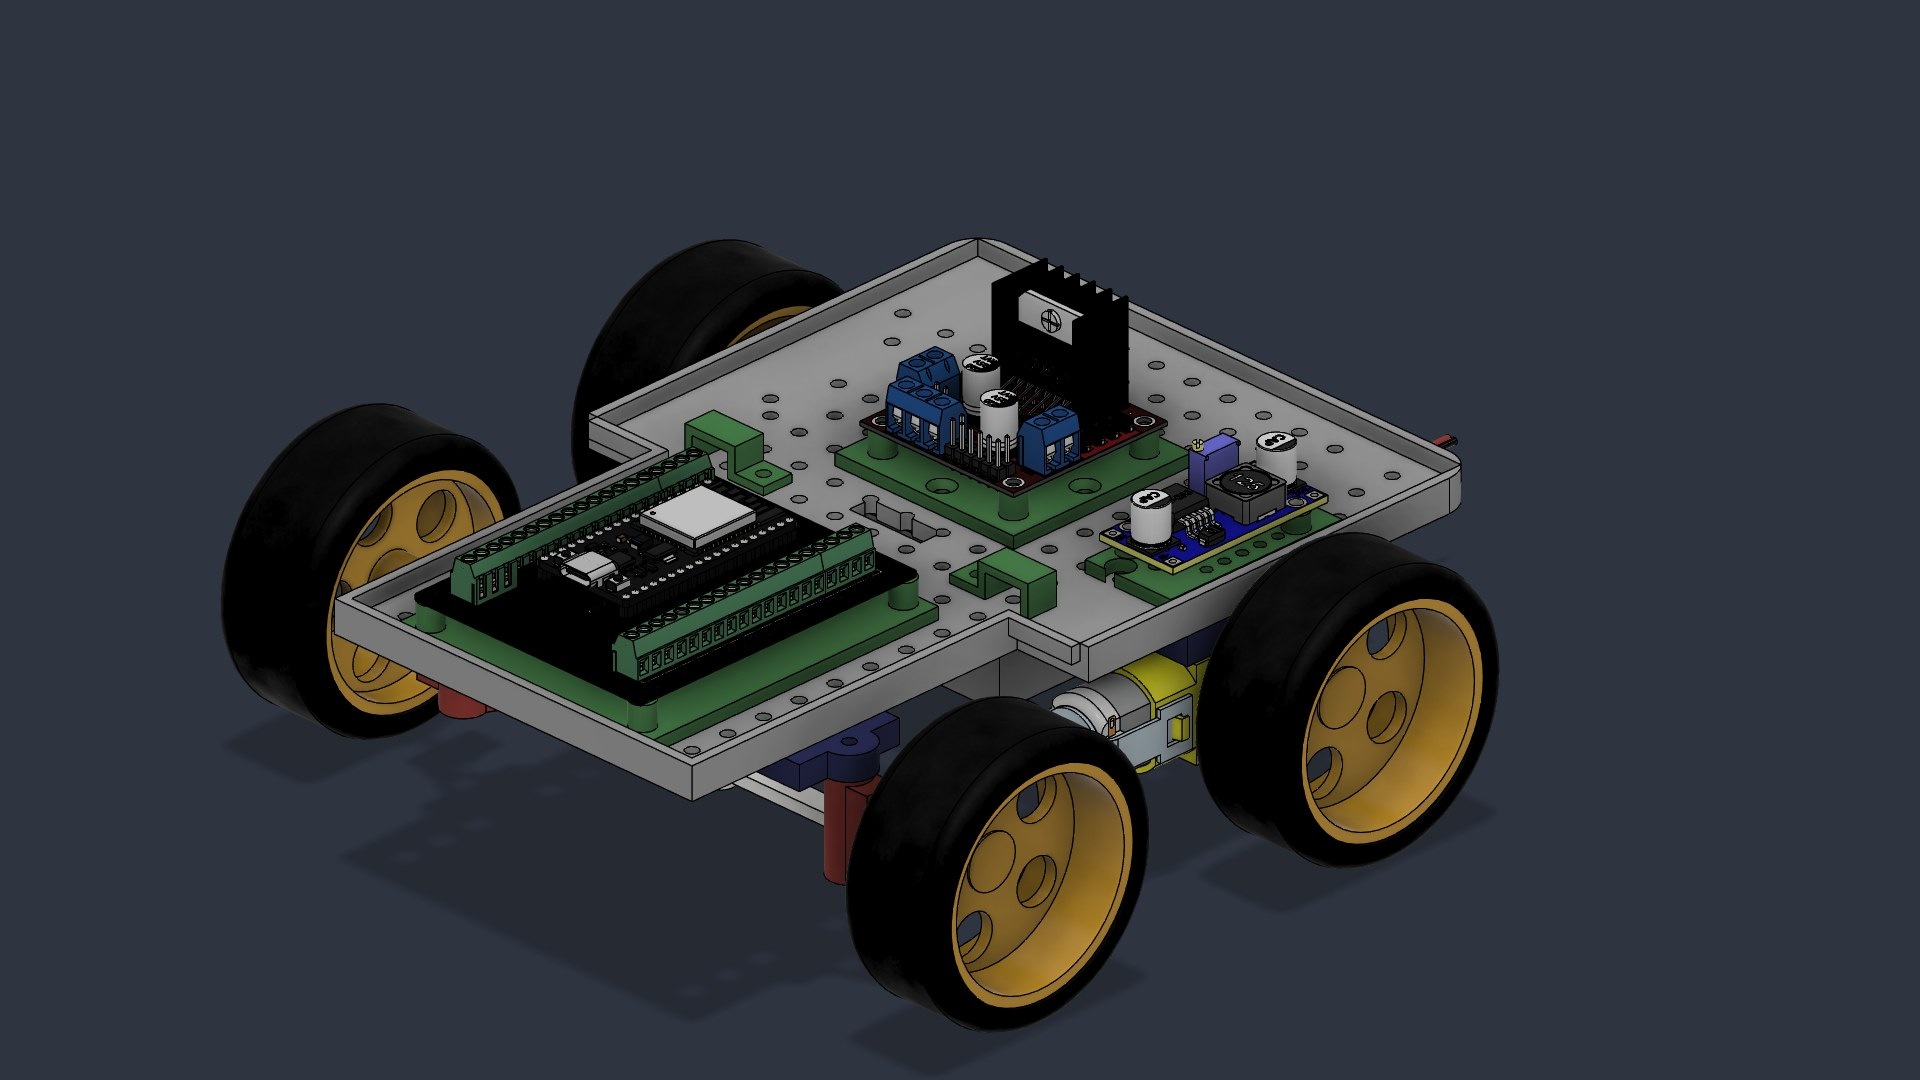
\includegraphics[width=\linewidth]{imagens/perspectiva_frente.jpg}\\[2pt]
\credito{Modelo 3D do carrinho, elaborado pela equipe}
\end{columns}
\end{frame}

\begin{frame}{Por que cibersegurança importa}
\begin{columns}[T]
\column{0.5\textwidth}
\begin{itemize}
  \item Quase tudo está conectado: geladeiras, portos, bancos, carros, hospitais
  \item Uma falha não fica só no computador: vira comida estragada, serviço parado ou dinheiro roubado
  \item A IA deixou ataques mais rápidos e baratos
\end{itemize}
\column{0.46\textwidth}
\begin{itemize}
  \item A maioria das invasões ainda começa no básico: senha padrão, sistema sem atualização, pessoa enganada
  \item Segurança não é só da equipe de TI: quem projeta, programa e usa também decide
\end{itemize}
\end{columns}
\ideia{Para quem projeta circuitos e sistemas controlados, segurança é requisito de projeto, como alimentação ou estabilidade.}
\end{frame}

\begin{frame}{Casos recentes: do digital ao físico}
\begin{columns}[T]
\column{0.32\textwidth}
\centering
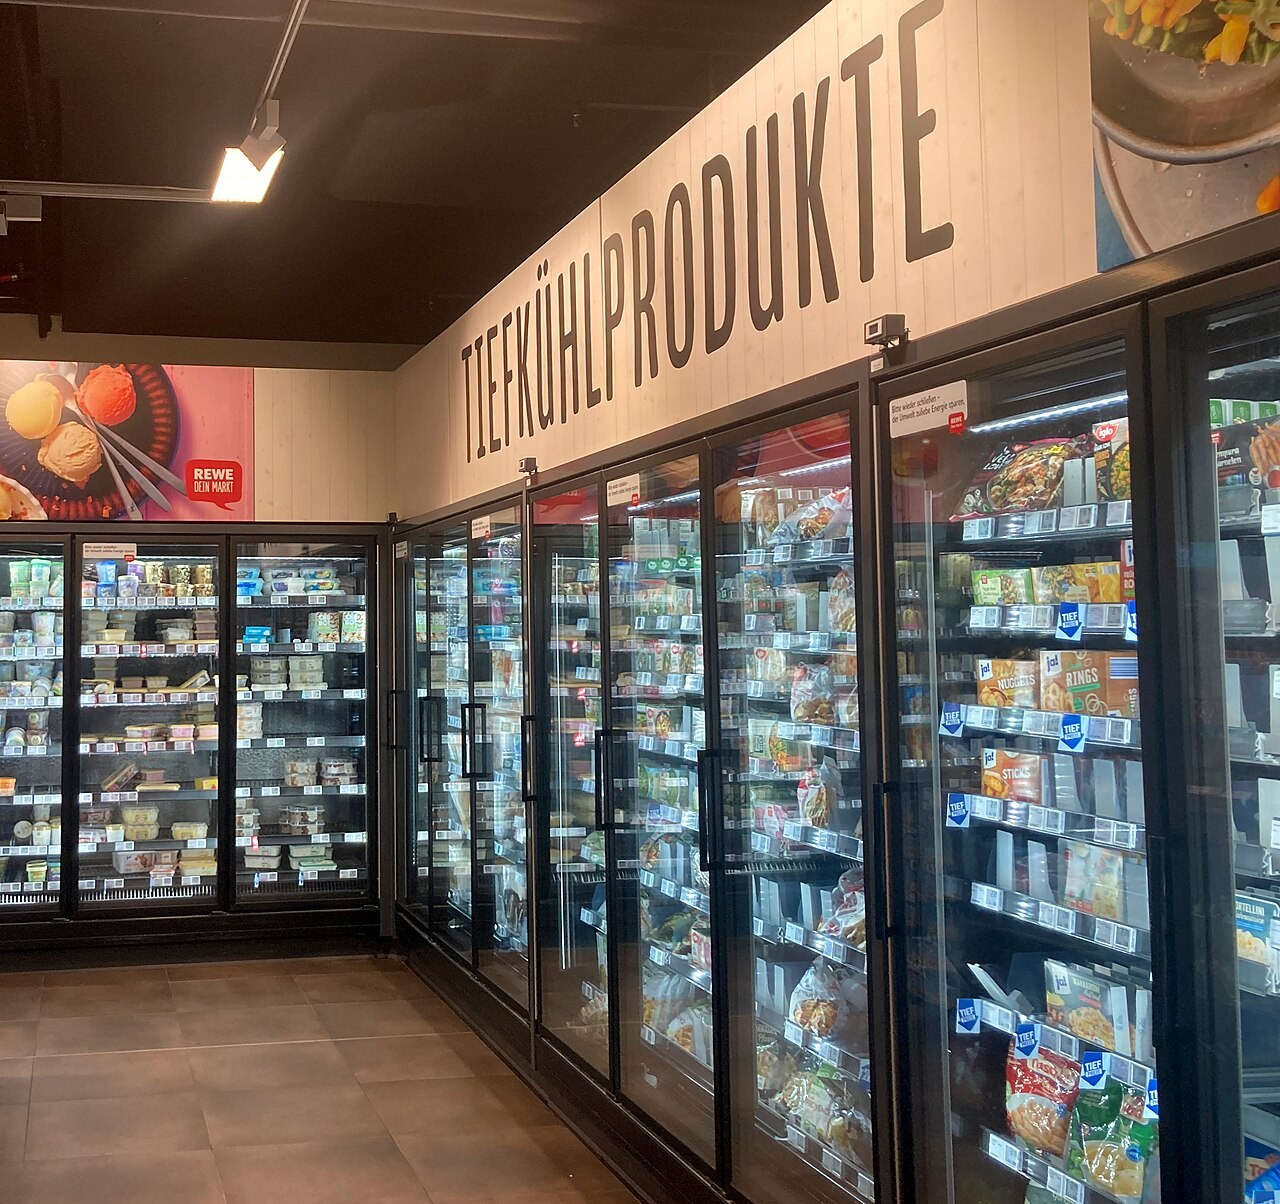
\includegraphics[width=\linewidth,height=2.3cm,keepaspectratio]{imagens/freezer_supermercado.jpg}\\
\credito{Ilustrativa: Alexis Jazz, CC BY 4.0, Wikimedia Commons}\\[2pt]
\footnotesize\textbf{Supermercados na Europa}\\out--nov/2026: freezers aquecidos a até 50~°C à distância
\column{0.32\textwidth}
\centering
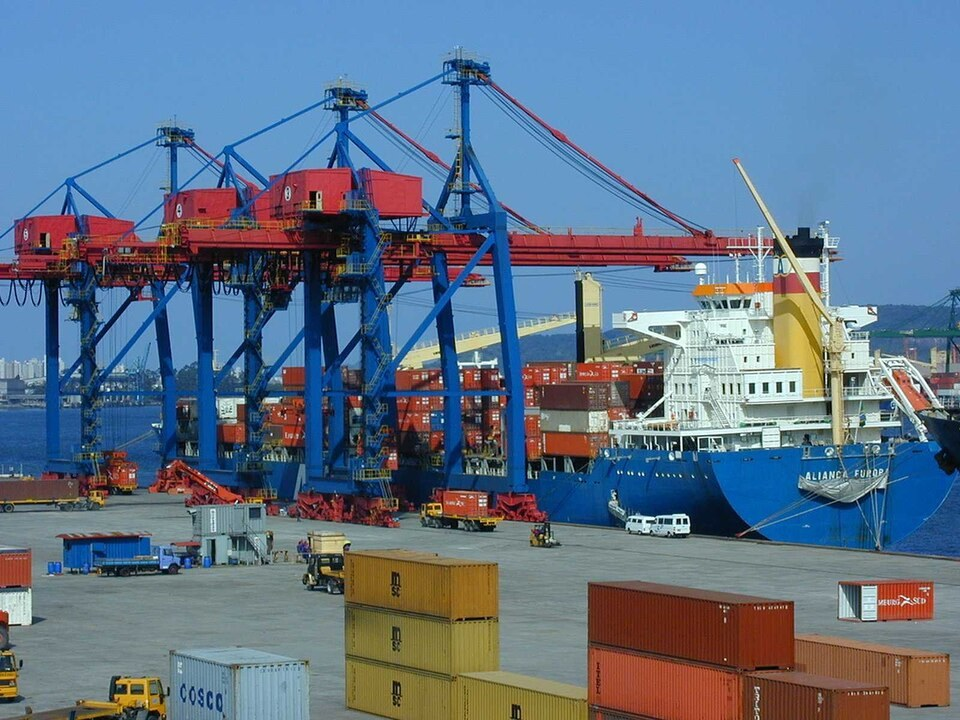
\includegraphics[width=\linewidth,height=2.3cm,keepaspectratio]{imagens/porto_santos.jpg}\\
\credito{Claus Bunks (Afrobrasil), CC BY 3.0, Wikimedia Commons}\\[2pt]
\footnotesize\textbf{Porto de Santos}\\6/nov/2026: sistemas fora do ar; navios e cargas seguiram por meios alternativos
\column{0.32\textwidth}
\centering

\includegraphics[width=\linewidth,height=2.3cm,keepaspectratio]{imagens/logo_binance.png}\\
\credito{Logo: Binance, domínio público}\\[2pt]
\footnotesize\textbf{Binance}\\29/out/2026: US\$~6,3 bi roubados; começou com uma entrevista de emprego falsa
\end{columns}
\ideia{Equipamento físico controlado pela rede, sistema que precisa operar sem rede e pessoas enganadas: os três aparecem no HIJACK.}
\end{frame}

\begin{frame}{A IA dos dois lados}
\begin{columns}[c]
\column{0.64\textwidth}
\footnotesize
\textbf{\color{vermelho}No ataque}
\begin{itemize}
  \item GTG-1002 (2025): o Claude Code atacou cerca de 30 organizações, fazendo de 80 a 90\% do trabalho
  \item Binance: ferramenta interna de IA usada para chegar às carteiras
  \item LiteLLM: pacote de IA adulterado roubando chaves (mar e out/2026)
\end{itemize}
\textbf{\color{verde}Na pesquisa e na defesa}
\begin{itemize}
  \item PHP2Shell (21/out): falhas antigas do PHP achadas com ajuda de IA
  \item Node.js: falha relatada pela segurança do OpenAI Codex
  \item Java4Shell (17/nov): prova de conceito criada com IA em cerca de 2~h
\end{itemize}
\column{0.32\textwidth}
\centering

\includegraphics[width=0.85\linewidth]{imagens/logo_anthropic.png}\\[8pt]

\includegraphics[height=0.75cm]{imagens/logo_php.png}\hspace{3pt}

\includegraphics[height=0.75cm]{imagens/logo_nodejs.png}\hspace{3pt}

\includegraphics[height=1.1cm]{imagens/java_duke.png}\\
\credito{Logos e mascote: Wikimedia Commons (domínio público, MIT e BSD)}
\end{columns}
\ideia{A IA encurta o tempo entre achar uma falha e explorá-la: atualizar rápido virou segurança.}
\end{frame}

\begin{frame}{A proposta}
\begin{columns}[c]
\column{0.5\textwidth}
\begin{itemize}
  \item Um carrinho com ESP32 pilotado pelo celular
  \item Uma equipe tenta tomar o controle; outra tenta defender
  \item Cada ataque tem efeito visível: o carrinho vira errado, anda de ré, para ou é sequestrado
  \item Rede local isolada; ataques simulados no próprio sistema
\end{itemize}
\column{0.46\textwidth}
\centering
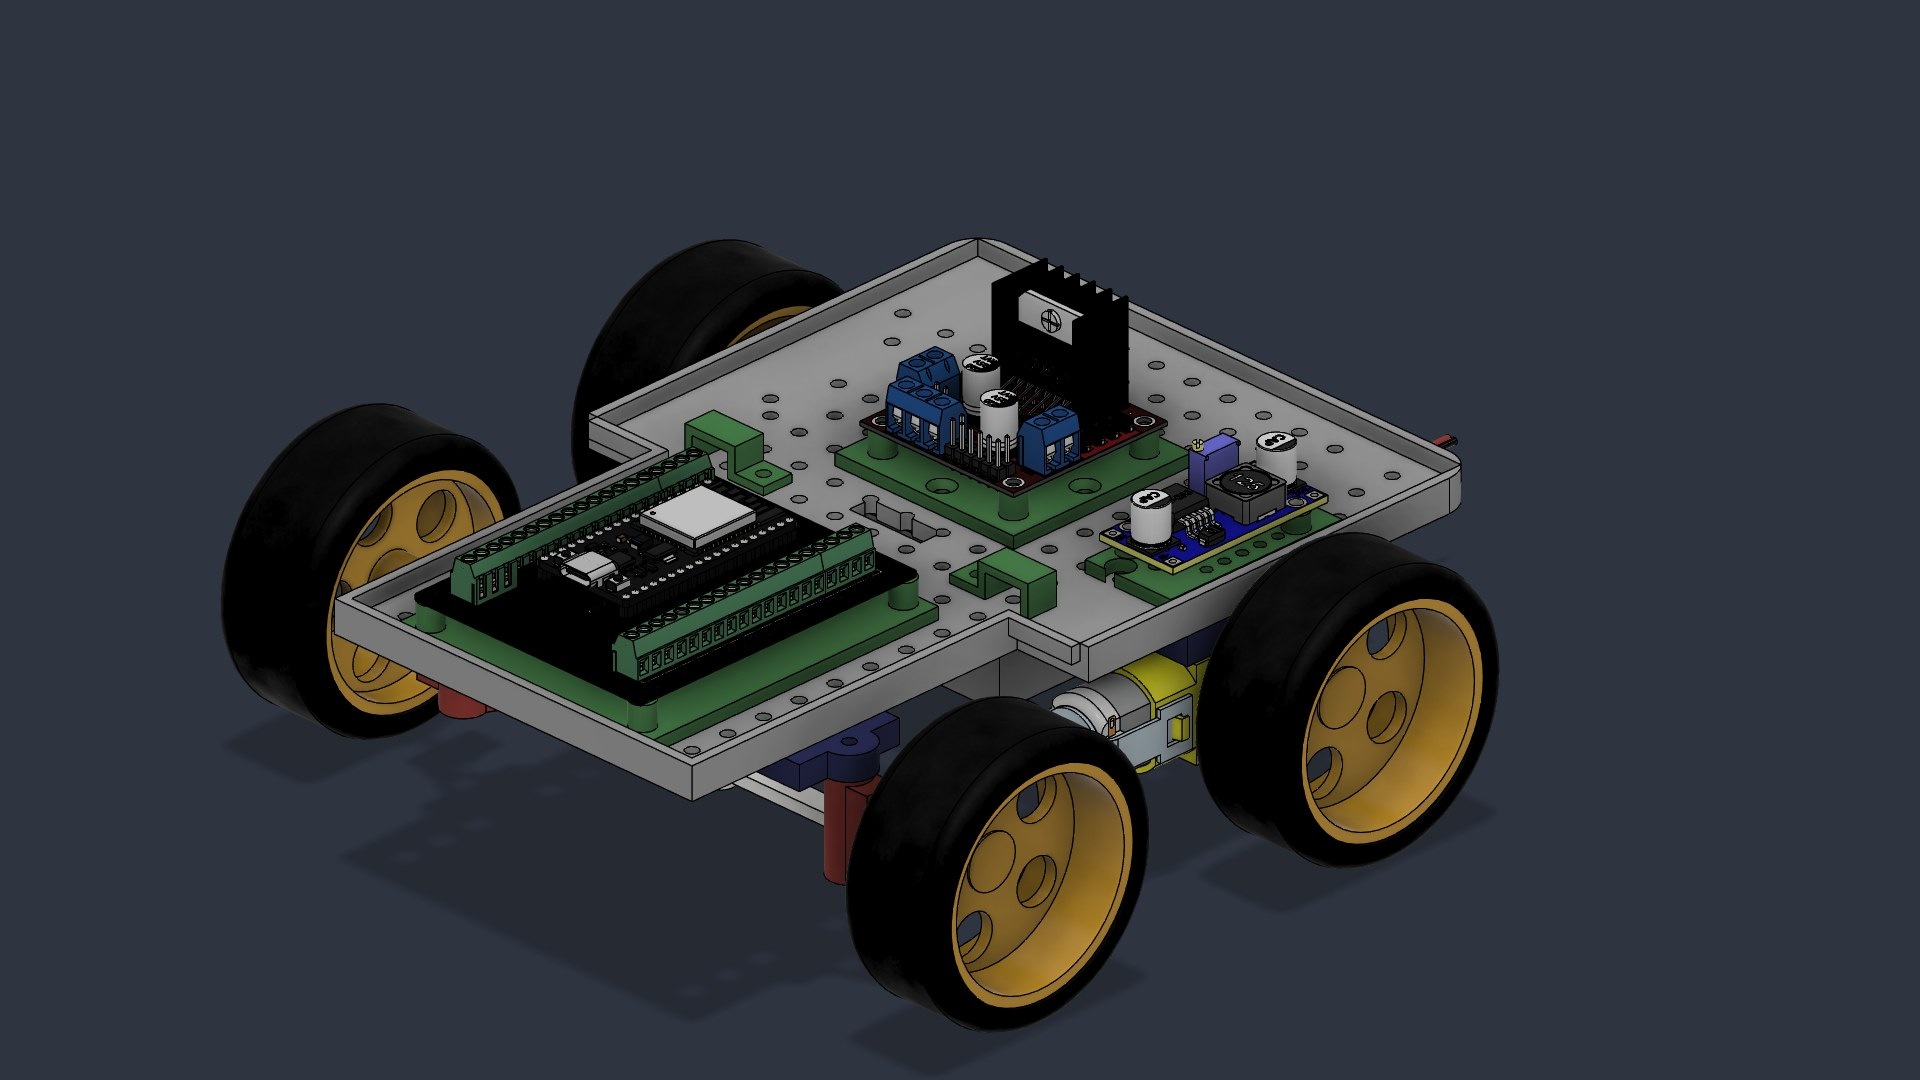
\includegraphics[width=\linewidth]{imagens/perspectiva_frente.jpg}\\
\credito{Modelo 3D do carrinho, elaborado pela equipe (Autodesk Fusion)}
\end{columns}
\ideia{Ataque costuma ser invisível. Aqui ele aparece no carrinho e no telão.}
\end{frame}

\begin{frame}{Objetivos de Desenvolvimento Sustentável (ODS)}
\centering
\begin{tikzpicture}[node distance=0.4cm]
\node[draw=none, fill={rgb,255:red,197;green,25;blue,45}, text=white, rounded corners, text width=3.85cm, minimum height=3.2cm, align=left, inner sep=6pt] (o4) {\textbf{\large ODS 4}\\\textbf{Educação de qualidade}\\[4pt]\footnotesize Meta 4.4: mais jovens e adultos com habilidades técnicas. O jogo ensina segurança na prática.};
\node[draw=none, fill={rgb,255:red,253;green,105;blue,37}, text=white, rounded corners, text width=3.85cm, minimum height=3.2cm, align=left, inner sep=6pt, right=of o4] (o9) {\textbf{\large ODS 9}\\\textbf{Indústria, inovação e infraestrutura}\\[4pt]\footnotesize Meta 9.1: infraestrutura confiável e resiliente. Equipamentos conectados precisam falhar com segurança.};
\node[draw=none, fill={rgb,255:red,0;green,104;blue,157}, text=white, rounded corners, text width=3.85cm, minimum height=3.2cm, align=left, inner sep=6pt, right=of o9] (o16) {\textbf{\large ODS 16}\\\textbf{Paz, justiça e instituições eficazes}\\[4pt]\footnotesize Meta 16.a: capacidade para prevenir e combater o crime, inclusive o digital.};
\end{tikzpicture}
\end{frame}

\begin{frame}{Papéis e modalidades}
\centering
\begin{tikzpicture}[node distance=0.5cm]
\node[caixa, text width=3.2cm, fill=verde!15] (p) {\textbf{Piloto}\\celular, joystick};
\node[caixa, text width=3.2cm, fill=verde!15, right=of p] (d) {\textbf{Hacker de defesa}\\liga as proteções};
\node[caixa, text width=3.2cm, fill=vermelho!15, right=of d] (a) {\textbf{Hacker de ataque}\\tenta tomar o controle};
\node[caixa, text width=3.2cm, below=0.6cm of d] (o) {\textbf{Operador e telão}\\conduz e mostra a partida};
\node[above=0.15cm of d, font=\small\bfseries, color=verde] {Equipe A};
\node[above=0.15cm of a, font=\small\bfseries, color=vermelho] {Equipe B};
\end{tikzpicture}
\vspace{0.3cm}
\begin{itemize}
  \item \textbf{1 carrinho}: no mínimo 3 jogadores (piloto, defesa e ataque)
  \item \textbf{2 carrinhos}: 4 jogadores; cada hacker ataca o adversário e defende o próprio
\end{itemize}
\ideia{Não há placar: o objetivo é ver o efeito de cada ataque e de cada defesa.}
\end{frame}

\begin{frame}{Como se joga}
\centering
\begin{tikzpicture}[node distance=0.25cm, every node/.style={font=\footnotesize}]
\node[caixa, text width=2.3cm] (s1) {\textbf{1. Largada}\\piloto dirige};
\node[caixa, text width=2.3cm, right=of s1] (s2) {\textbf{2. Invasão}\\4 etapas guiadas};
\node[caixa, text width=2.3cm, right=of s2, fill=vermelho!15] (s3) {\textbf{3. Ataque}\\carrinho sai do controle};
\node[caixa, text width=2.3cm, right=of s3, fill=verde!15] (s4) {\textbf{4. Defesa}\\proteções ligadas};
\node[caixa, text width=2.3cm, right=of s4] (s5) {\textbf{5. Fim}\\métricas};
\draw[seta] (s1) -- (s2); \draw[seta] (s2) -- (s3); \draw[seta] (s3) -- (s4); \draw[seta] (s4) -- (s5);
\end{tikzpicture}
\vspace{0.4cm}
\begin{itemize}
  \item Invasão: escanear, identificar o alvo, explorar a falha e modificar comandos
  \item A senha começa como \texttt{1234}, de propósito
  \item O telão compara o comando pedido pelo piloto com o que o carrinho recebeu
\end{itemize}
\ideia{O público vê \enquote{comando alterado no caminho} quando o ataque funciona.}
\end{frame}

\begin{frame}{Ataques e defesas do jogo}
\footnotesize
\begin{tabularx}{\textwidth}{@{}p{2.1cm}L>{\raggedright\arraybackslash}p{4.4cm}@{}}
\toprule
\textbf{Grupo} & \textbf{Ataques (12 no total)} & \textbf{Defesa} \\
\midrule
Sabotagem & Inverter frente/ré e esquerda/direita, viés e travamento da direção & Integridade (simulada) \\
 & Replay: repete comandos antigos & Proteção contra repetição (simulada) \\
 & Atraso e perda de pacotes & Nenhuma: o carrinho para sozinho \\
Espionagem & Interceptar o tráfego & Criptografia (simulada) \\
 & Quebrar a senha com lista de senhas comuns & \textbf{Trocar a senha padrão (real)} \\
Canal & Derrubar o link por 5~s & Nenhuma: o carrinho para sozinho \\
 & Telemetria falsa & Integridade (simulada) \\
Controle & \alert{Sequestro}: o atacante dirige o carrinho & \textbf{Trocar a senha padrão (real)} \\
\bottomrule
\end{tabularx}
\ideia{Trocar a senha não impede as inversões: ela barra quem não tem acesso, não a alteração no caminho.}
\end{frame}

\begin{frame}{Arquitetura}
\centering
\begin{tikzpicture}[font=\footnotesize]
\node[caixa, text width=2.2cm] (piloto) at (0,2.1) {Celular (piloto)};
\node[caixa, text width=2.2cm] (hacker) at (0,0.95) {Notebooks (hackers)};
\node[caixa, text width=2.2cm] (oper) at (0,-0.2) {Operador};
\node[caixa, text width=2.2cm] (telao) at (0,-1.35) {Telão};
\node[caixa, text width=3.2cm, minimum height=4.3cm, fill=verde!10] (srv) at (4.6,0.37) {\textbf{Servidor}\\[2pt]sessões e permissões\\ataques e defesas\\controle do carrinho\\simulador};
\node[caixa, text width=2.2cm] (esp) at (9.3,0.37) {ESP32 (firmware)};
\node[caixa, text width=2.2cm] (mot) at (9.3,2.1) {L298N e motores TT};
\node[caixa, text width=2.2cm] (servo) at (9.3,-1.35) {Servo SG90};
\draw[seta, <->] (piloto) -- (srv.west |- piloto);
\draw[seta, <->] (hacker) -- (srv.west |- hacker);
\draw[seta, <->] (oper) -- (srv.west |- oper);
\draw[seta] (srv.west |- telao) -- (telao);
\draw[seta, <->] (srv) -- node[above, font=\scriptsize]{WebSocket} node[below, font=\scriptsize]{Wi-Fi} (esp);
\draw[seta] (esp) -- node[right, font=\scriptsize]{PWM} (mot);
\draw[seta] (esp) -- node[right, font=\scriptsize]{PWM 50 Hz} (servo);
\end{tikzpicture}
\ideia{O navegador nunca fala direto com o carrinho: tudo passa pelo servidor, que é quem aplica os ataques e as defesas.}
\end{frame}

\begin{frame}{Componentes}
\begin{columns}[T]
\column{0.32\textwidth}
\centering
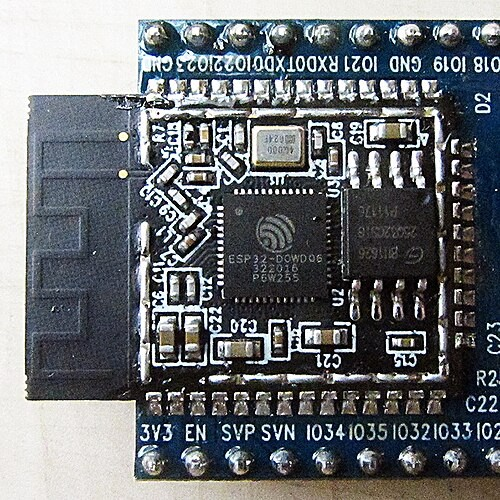
\includegraphics[height=2.4cm]{imagens/esp32.jpg}\\
\textbf{ESP32-WROOM-32}\\\small Wi-Fi e dois núcleos\\
\credito{Brian Krent, CC BY-SA 4.0, Wikimedia Commons}
\column{0.32\textwidth}
\centering
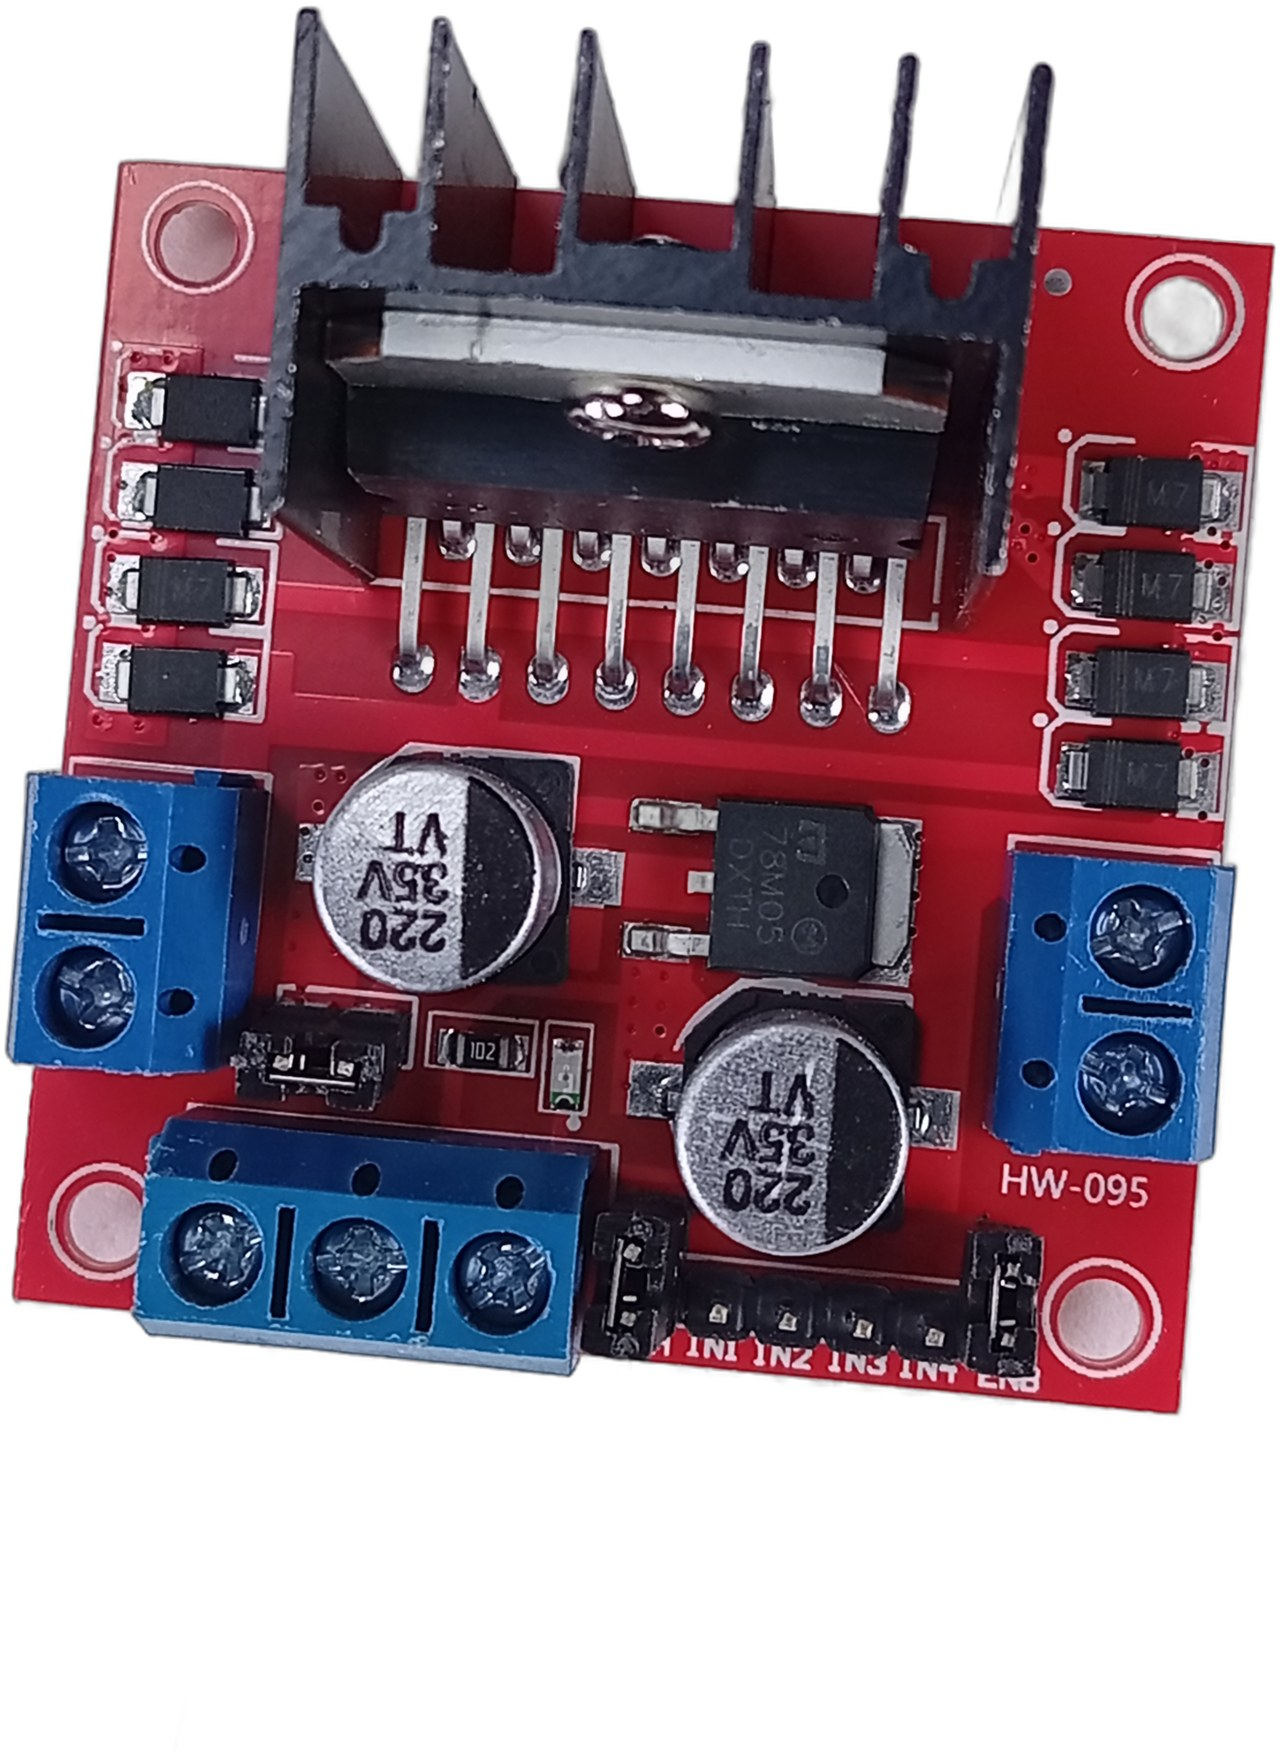
\includegraphics[height=2.4cm]{imagens/l298n.jpg}\\
\textbf{Ponte H L298N}\\\small sentido e velocidade dos motores\\
\credito{Luiz Augusto S. de Mesquita, CC0, Wikimedia Commons}
\column{0.32\textwidth}
\centering
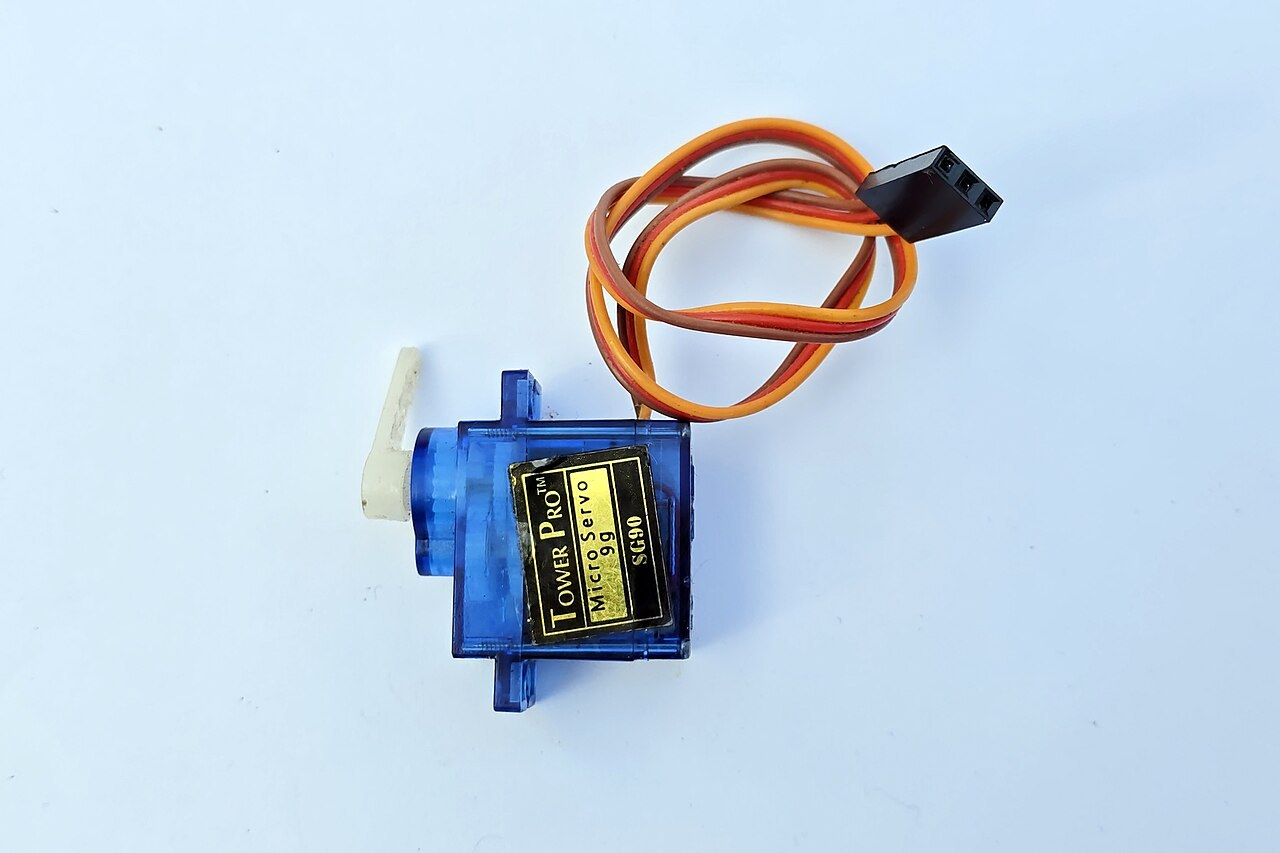
\includegraphics[height=2.4cm]{imagens/sg90.jpg}\\
\textbf{Servo SG90}\\\small direção das rodas da frente\\
\credito{Suyash Dwivedi, CC BY-SA 4.0, Wikimedia Commons}
\end{columns}
\vspace{0.3cm}
\small Também: 2 motores TT amarelos com redução 1:48 (3 a 6~V), regulador LM2596 ajustado em 5~V, 2 baterias 18650 em série (7,4~V) e estrutura projetada pela equipe e impressa em 3D.
\ideia{Fotos ilustrativas dos mesmos modelos de peça usados no carrinho.}
\end{frame}

\begin{frame}{Direção}
\begin{columns}[c]
\column{0.5\textwidth}
\begin{itemize}
  \item Servo move uma alavanca e duas barras (Ackermann simplificado)
  \item Comando de $-100\%$ a $+100\%$ vira até $\pm45^\circ$ no servo
  \item Limite abaixo do batente mecânico ($\approx48^\circ$)
  \item Raio de curva previsto: cerca de 27~cm
\end{itemize}
\column{0.46\textwidth}
\centering
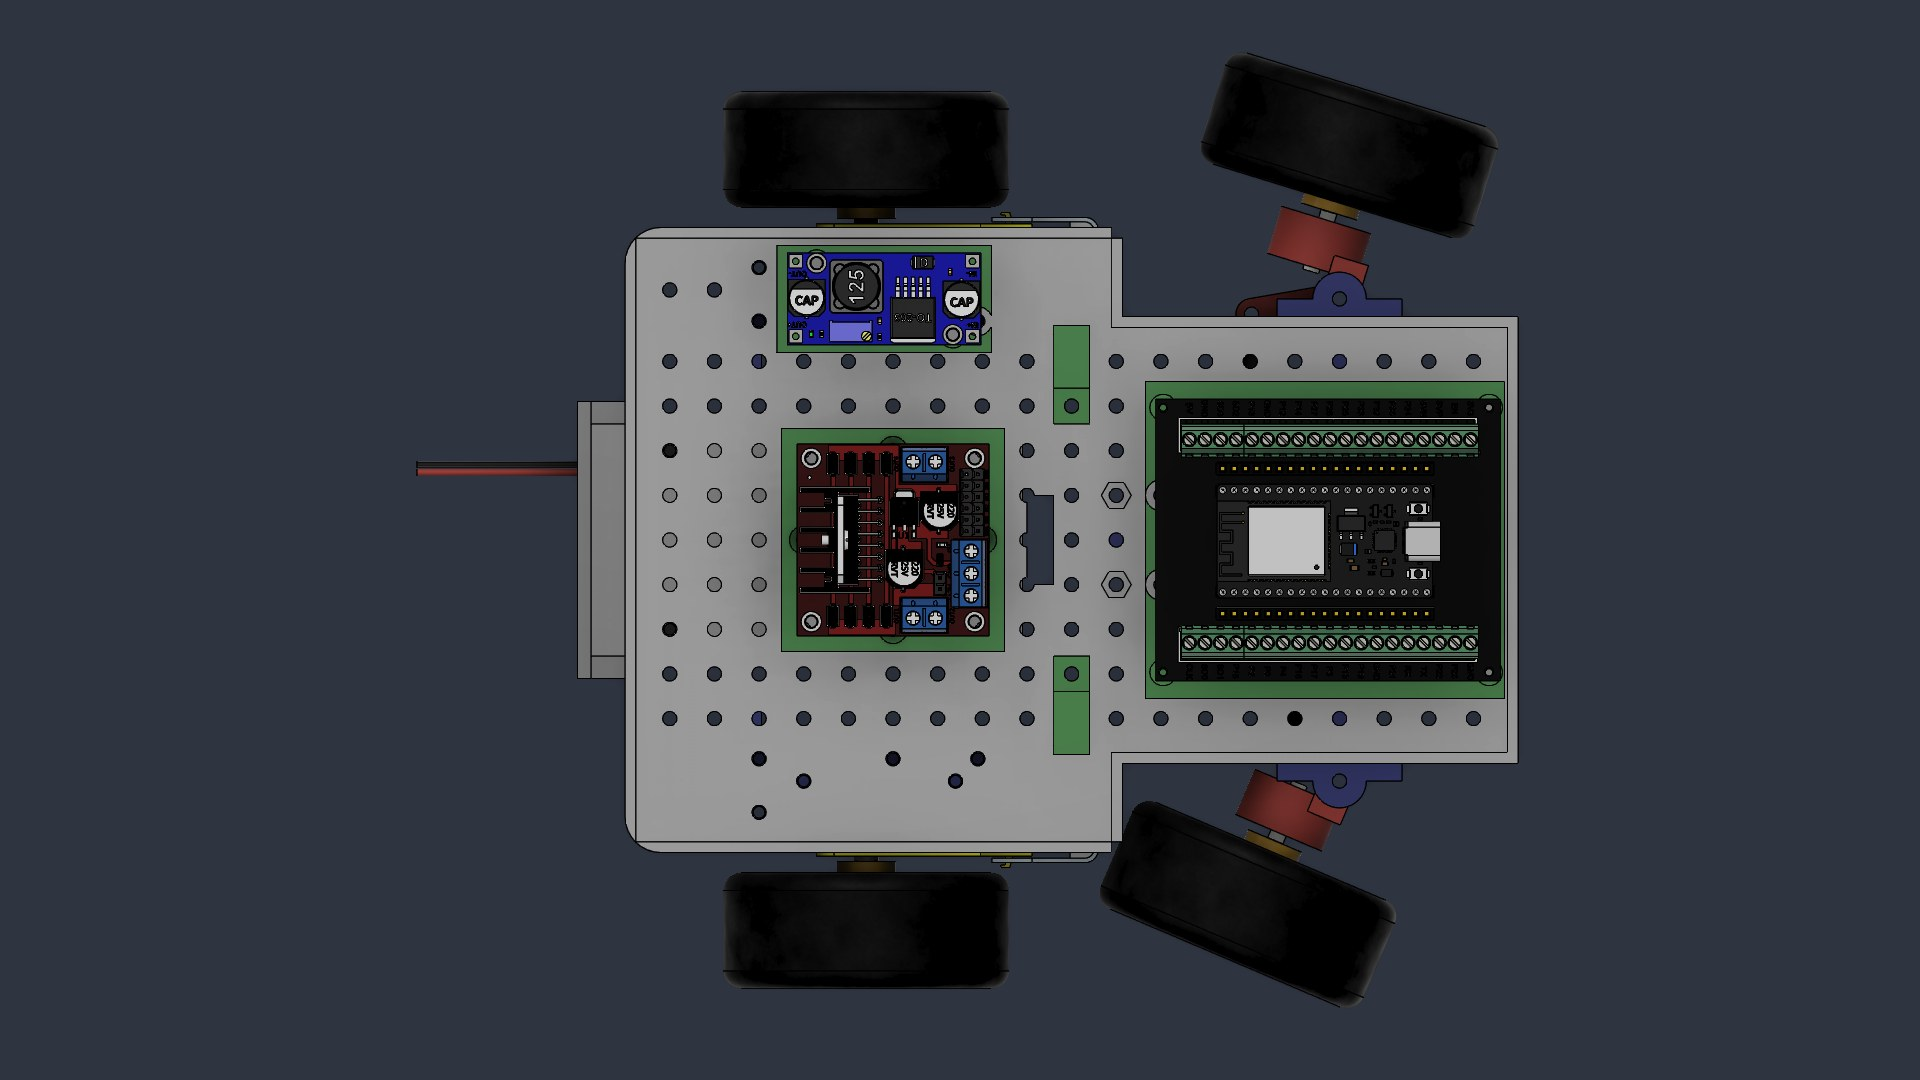
\includegraphics[width=\linewidth]{imagens/curva_direita.jpg}\\
\credito{Modelo 3D: servo a 45°, roda interna $\approx23^\circ$, externa $\approx17^\circ$}
\end{columns}
\ideia{Na curva, a roda de dentro esterça mais que a de fora, como em um carro de verdade.}
\end{frame}

\begin{frame}{Alimentação e PWM}
\begin{columns}[T]
\column{0.5\textwidth}
\begin{itemize}
  \item Bateria 7,4~V (8,4~V cheia) $\rightarrow$ L298N $\rightarrow$ motores
  \item Bateria $\rightarrow$ regulador 5~V $\rightarrow$ ESP32 e servo
  \item GND comum a todos
  \item Controle em malha aberta: sem sensores de velocidade
\end{itemize}
\column{0.46\textwidth}
\begin{block}{Por que o PWM vai só até 80\%}
\[
V_{\text{motor}} \approx (8{,}4 - 2) \times 0{,}8 \approx 5{,}1~\text{V}
\]
\small A L298N perde cerca de 2~V; os motores são de até 6~V.
\end{block}
\end{columns}
\ideia{O PWM liga e desliga o motor muito rápido; a fração do tempo ligado define a tensão média.}
\end{frame}

\begin{frame}{Comunicação ESP32 e servidor}
\begin{columns}[T]
\column{0.52\textwidth}
\small
\begin{enumerate}
  \item ESP32 se identifica com um segredo
  \item Servidor manda comandos numerados: tração, direção e validade de 400~ms
  \item ESP32 confirma o que aplicou
  \item Telemetria a cada 500~ms
\end{enumerate}
\column{0.44\textwidth}
\begin{block}{Parada segura}
\small
\begin{itemize}
  \item Soltar o joystick: para na hora
  \item Sem comando novo em 400~ms: para sozinho
  \item Vale no servidor e no ESP32
\end{itemize}
\end{block}
\end{columns}
\ideia{Os ataques acontecem no servidor. Para o ESP32, um ataque é só um comando diferente ou um comando que não chega.}
\end{frame}

\begin{frame}{Resultados}
\begin{columns}[T]
\column{0.5\textwidth}
\begin{itemize}\small
  \item \textbf{343} testes automatizados aprovados
  \item \textbf{57} testes no navegador aprovados (1 pulado)
  \item ESP32 real: \textbf{23 de 23} verificações
  \item Bancada com motores: \textbf{17 de 18}, ajuste na perda de pacotes, depois \textbf{18 de 18}
\end{itemize}
\column{0.46\textwidth}
\small
\begin{tabular}{@{}lr@{}}
\toprule
\textbf{Teste na bancada} & \textbf{Parada} \\
\midrule
Soltar o joystick & 149~ms \\
Link derrubado & 124~ms \\
STOP ALL no sequestro & 102~ms \\
\bottomrule
\end{tabular}
\end{columns}
\ideia{O primeiro 17 de 18 foi útil: mostrou que a perda de pacotes sorteada um a um não parava o carrinho, e mudamos para perdas em rajadas.}
\end{frame}

\begin{frame}{Limitações e próximos passos}
\begin{itemize}
  \item Peças impressas, mas o carrinho ainda não foi montado nem testado no chão
  \item Testes com fonte de bancada; as baterias ainda não foram usadas
  \item Sem fusível e sem proteção da bateria (decisão da equipe)
  \item Ajustar a polaridade de um motor e refazer a alimentação do ESP32
  \item Rede aberta, sem TLS: só em laboratório isolado
\end{itemize}
\ideia{Fomos honestos no relatório: só dizemos que funcionou onde testamos de verdade.}
\end{frame}

\begin{frame}{Conclusão}
\begin{itemize}
  \item A IA acelera ataque e defesa: invasões, descoberta de falhas e provas de conceito em horas
  \item As defesas básicas continuam decisivas: trocar senha padrão, atualizar rápido, desconfiar do que se instala
  \item Equipamentos precisam falhar de forma segura
  \item O HIJACK transforma essas ideias em algo que se vê
\end{itemize}
\ideia{E a IA também ajudou a construir este projeto, sob revisão da equipe.}
\end{frame}

\begin{frame}[standout]
Obrigado!\\[0.5em]
\normalsize Perguntas?
\end{frame}

\begin{frame}[allowframebreaks]{Referências}
\tiny
\begin{itemize}
  \item ANTHROPIC. \emph{Disrupting the first reported AI-orchestrated cyber espionage campaign}. Nov. 2025.
  \item SABIN, S. Chinese hackers used Anthropic's AI agent to automate spying. \emph{Axios}, 13 nov. 2025.
  \item FAUSTINO, F. Hackers usaram IA da Anthropic em ciberataque global. \emph{Tecnoblog}, 14 nov. 2025.
  \item HELP NET SECURITY. LiteLLM PyPI packages compromised in expanding TeamPCP supply chain attacks. 25 mar. 2026.
  \item BLEEPINGCOMPUTER. LiteLLM release pipeline hacked to distribute info-stealer malware. 22 out. 2026.
  \item WIZ RESEARCH. PHP2Shell: AI uncovers critical RCE vulnerabilities affecting 70\% of the Internet. 21 out. 2026.
  \item ALURA. PHP2Shell: quando uma requisição basta para dominar um servidor. 30 out. 2026.
  \item BLEEPINGCOMPUTER. GitLab warns of new max severity code execution vulnerability. 22 out. 2026.
  \item NODE.JS. Wednesday, October 21, 2026 security releases. 21 out. 2026.
  \item REUTERS. Binance: hackers used fake job interview before \$6.3 billion hack. \emph{NBC News}, 3 nov. 2026.
  \item STARTSE. IA e entrevista de emprego falsa: o que está por trás do ataque à Binance. 4 nov. 2026.
  \item AL JAZEERA. Very cold war: who's attacking Europe's supermarket freezers? 3 nov. 2026.
  \item ANDRADE, B. Hackers sabotam freezers de supermercados na Europa. \emph{Tecnoblog}, 2 nov. 2026.
  \item SBT NEWS. Porto de Santos confirma que sofreu ataque hacker. 10 nov. 2026.
  \item NUNES, V. PF abre inquérito para investigar ataque hacker contra sistemas do Porto de Santos. \emph{CartaCapital}, 10 nov. 2026.
  \item MADEIRA, L. Porto de Santos recupera 70\% dos backups após ataque hacker. \emph{Times Brasil}, 12 nov. 2026.
  \item WIZ RESEARCH. CVE-2026-114938 OpenJDK RCE (Java4Shell): everything you need to know. 17 nov. 2026.
  \item TENABLE. Java4Shell (CVE-2026-114938): frequently asked questions. 17 nov. 2026.
\end{itemize}
\textbf{Imagens}: Wikimedia Commons (autores e licenças indicados em cada slide); modelo 3D do carrinho elaborado pela equipe no Autodesk Fusion.
\end{frame}

\end{document}
